%!TEX program = xelatex
%!TEX option = --output-driver="xdvipdfmx -V7"
\documentclass[12pt,hyperref={CJKbookmarks=true}]{beamer}
\usetheme{CambridgeUS}
\usecolortheme{dolphin}
\usefonttheme{professionalfonts}
\setbeamertemplate{bibliography item}{}
\usepackage{lmodern}
\graphicspath{{figure/}}

\usepackage{amsmath,amssymb,esint} 
\allowdisplaybreaks[0]
\usepackage{siunitx}
\usepackage{graphicx} 
\usepackage{array} 
\usepackage{multirow} 
\usepackage{braket}

\newcommand{\dif}{\,\mathrm d}
\newcommand\mi{\mathrm{i}}
\newcommand\e{\mathrm{e}}
\newcommand{\rf}{\text{rf}}
\newcommand{\thm}{\text{th}}
\DeclareMathOperator{\Hc}{H.c.}

% \usepackage[style=authoryear-comp,sorting=none]{biblatex}
% \bibliography{photonnumber}
\bibliographystyle{unsrt}

\title[Nature 445, 515-518]{Resolving photon number states in a superconducting circuit}
\author[Ming, Elena]{Ming Lyu, Elena de la Hoz Lopez-Collado}
\institute[Princeton]{Final projects for ELE456 at Princeton}
\date{May 11, 2017}
\begin{document}
\begin{frame}
\titlepage
\end{frame}
\begin{frame}
    \tableofcontents
\end{frame}

\section{Introduction} 
\begin{frame}[t]\frametitle{The paper}
    
This is for paper \cite{schuster2007resolving} % To show bib

\end{frame}

\section{Experiment implementation}

\section{The model}
\subsection{Diagonal under strong dispersive limit}
\subsection{Rotating wave approximation}
\subsection{Dissipation: the collapse operators}
\subsection{Measurement}
\begin{frame}[t]\frametitle{Measurement}
In the experiment, the transmitted amplitude at frequency $\omega_{\rf}$ is the main observable. The exact way to measure it is not mentioned in this paper, 
but can be check in Schuster's thesis: \cite{schuster2007circuit}. 
\begin{center}
  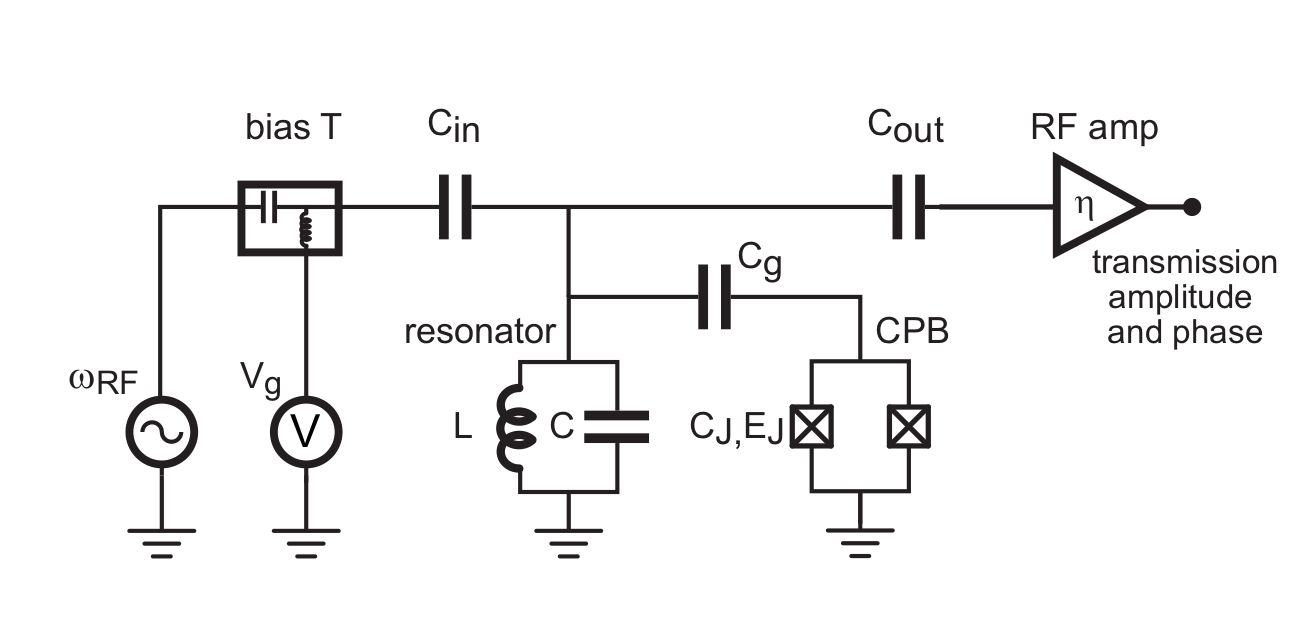
\includegraphics[width=0.6\textwidth]{measurement.png}
\end{center}
	\begin{itemize}
		\item What we really measure is the expectation of the voltage, or 
		electrical field $E\propto\langle a + a^\dag \rangle$
	\end{itemize}

\end{frame}

\section{Numerical simulation}
\subsection{Property of the cavity}
\begin{frame}[t]\frametitle{Property of the cavity: Analytical}
\begin{itemize}
	\item Without the qubit, the cavity state is equivalently a damped harmonic oscillator with driving
	$$
	 H = \delta a^\dag a + \epsilon (a + a^\dag)
	$$
	Collapse operators: $\sqrt{\kappa(n_{\thm}+1)}a$ and 
	$\sqrt{\kappa n_{\thm}}a^\dag$
	\item When it's off resonant, its steady state is not but approximately a coherent state
	\item Analytically the photon number expectation value is 
	$$
	\bar n = \frac{\epsilon^2}{\delta^2 + \kappa^2/4} + n_{\thm}
	$$
\end{itemize}
\end{frame}

\begin{frame}[t]\frametitle{Property of the cavity: Numerical}
\begin{itemize}
	\item Numerically, a truncate on Fock space is needed
	\item To check the validity of the truncate, we plot the photon distribution 
	and frequency response of the cavity. 
\end{itemize}
\begin{columns}
\begin{column}{0.5\linewidth}
	\centering
    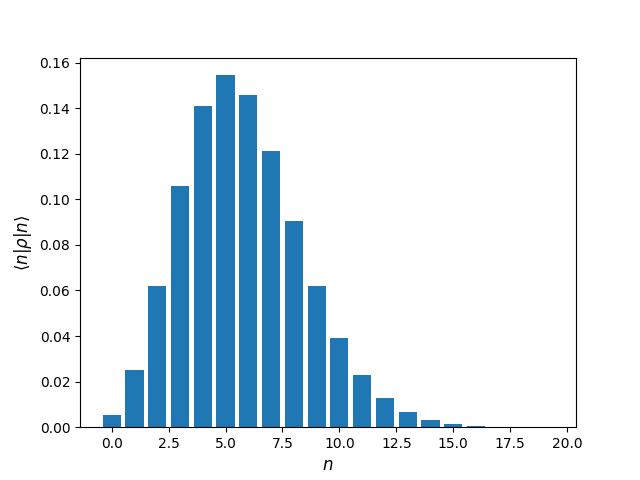
\includegraphics[width=\textwidth]{photon_number_dist.png}
\end{column}%
\begin{column}{0.5\linewidth}
	\centering
    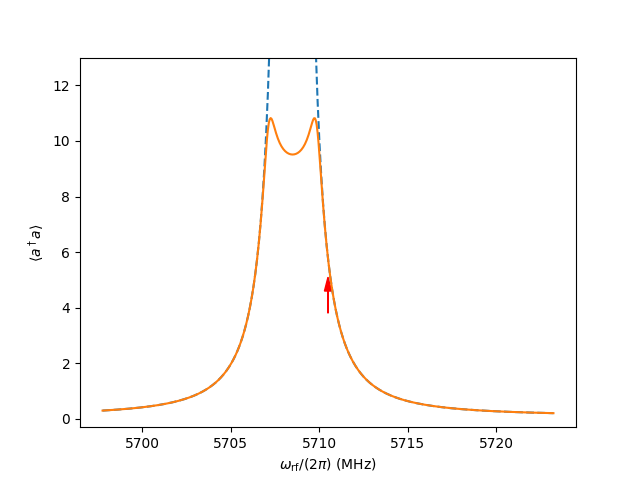
\includegraphics[width=\textwidth]{resonance.png}
\end{column}
\end{columns}
\end{frame}

\subsection{Reproduce results}
\begin{frame}[t]\frametitle{Direct spectroscopic observation of quantized cavity photon number}
\begin{columns}
\begin{column}{0.4\linewidth}
\begin{itemize}
	\item For a fixed driving $\epsilon_{\rf}$, plot the reduction
	$V_0 - \langle a^\dag + a\rangle_{ss}$ v.s. $\omega_{s}$. 
	\begin{equation*}
		\bar n = n_{\thm} + \frac{\epsilon_{\rf}^2}{\delta^2 + \kappa^2/4}
	\end{equation*}
\end{itemize}
\end{column}%
\begin{column}{0.6\linewidth}
	\centering
    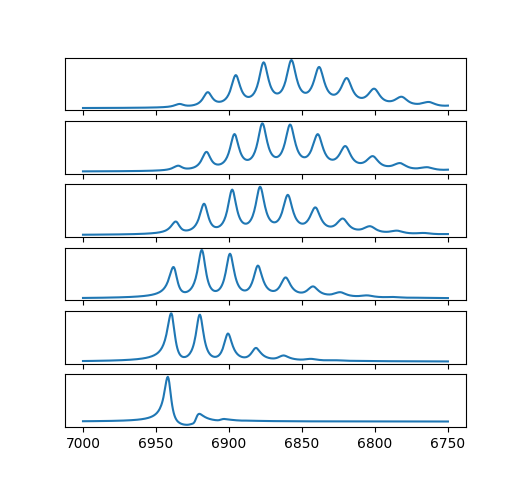
\includegraphics[width=\textwidth]{sweaping.png}
\end{column}
\end{columns}
\end{frame}

\begin{frame}[t]
\begin{columns}
\begin{column}{0.35\linewidth}
    \centering
    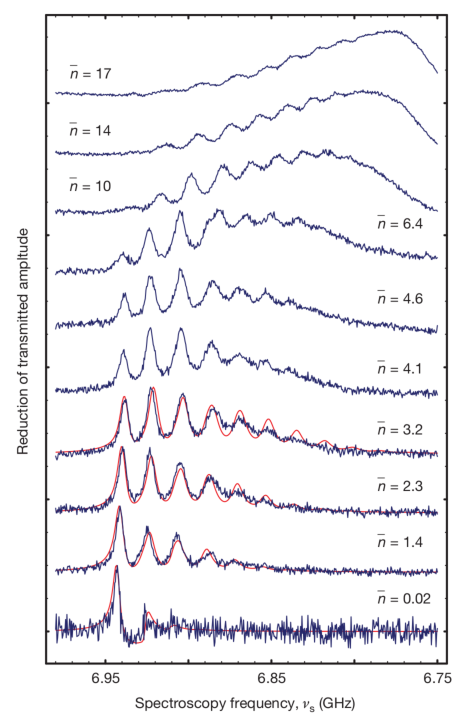
\includegraphics[width=\linewidth]{sweaping_origin.pdf}
    % \caption{Original results (theory: red lines)}
\end{column}%
\begin{column}{0.65\linewidth}
	\centering
    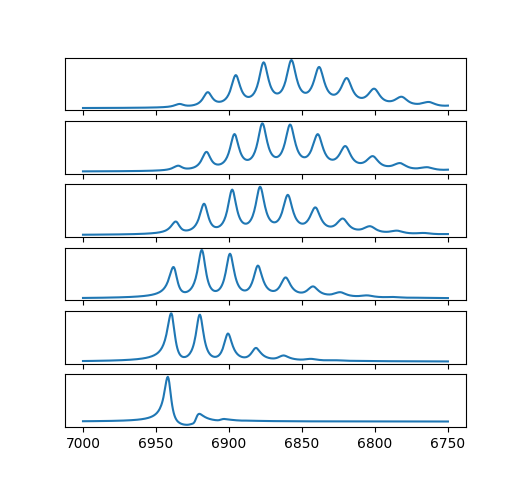
\includegraphics[width=\linewidth]{sweaping.png}
\end{column}
\end{columns}
\begin{itemize}
	\item The way $\bar n$ is defined is larger than ours. 
\end{itemize}
\end{frame}

\begin{frame}[t]\frametitle{Thermal Drive}
    
\begin{columns}
\begin{column}{0.4\linewidth}
\begin{itemize}
	\item Thermal Drive is equivalent to setting $n_{\thm}$ in collapse operator
	to the driving average, with small $\epsilon_{\rf}$ to show the phase 
	lock-in at the given frequency. 
\end{itemize}
\end{column}%
\begin{column}{0.6\linewidth}
	\centering
    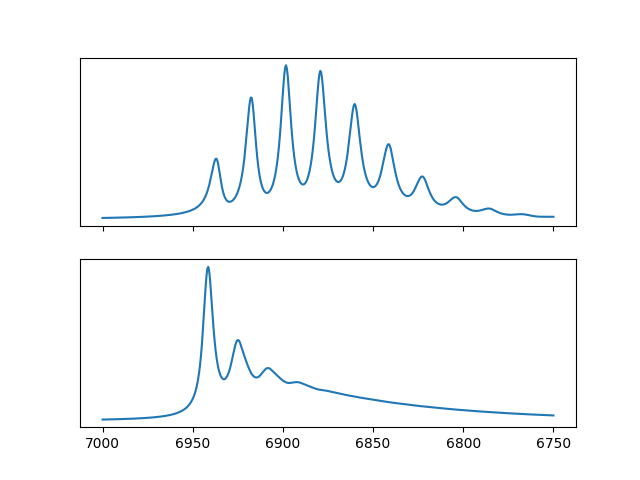
\includegraphics[width=\textwidth]{thermal.png}
\end{column}
\end{columns}
\end{frame}

\begin{frame}[t]
\begin{columns}
\begin{column}{0.4\linewidth}
    \centering
    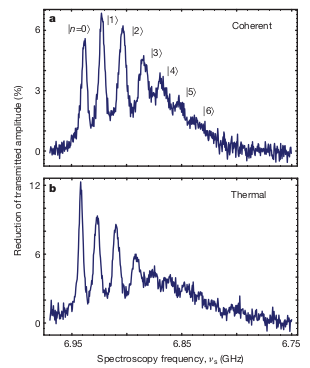
\includegraphics[width=\linewidth]{thermal_origin.png}
    % \caption{Original results (theory: red lines)}
\end{column}%
\begin{column}{0.6\linewidth}
	\centering
    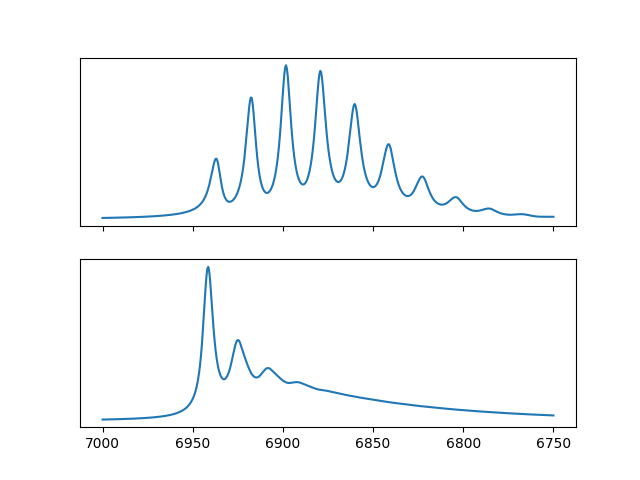
\includegraphics[width=\linewidth]{thermal.png}
\end{column}
\end{columns}
\begin{itemize}
	\item Note that there's no thermal drive theory fitting. 
	Our results tracks fewer peaks, but this depends on 
	how they do the measurement, which is not mentioned in the paper. 
\end{itemize}
\end{frame}

\section{Discussion}
\begin{frame}[t]\frametitle{Discussion: The picture of what happens}
\begin{itemize}
	\item The peaks shows discreteness in the photon state in the cavity. 
	\item Exciting the qubit making the cavity off-resonance, which results in
	the reduction? \pause \textbf{NOT TRUE} \pause
	\item Expected photon number increases at the peaks!
\begin{columns}
\begin{column}{0.5\linewidth}
    \centering
    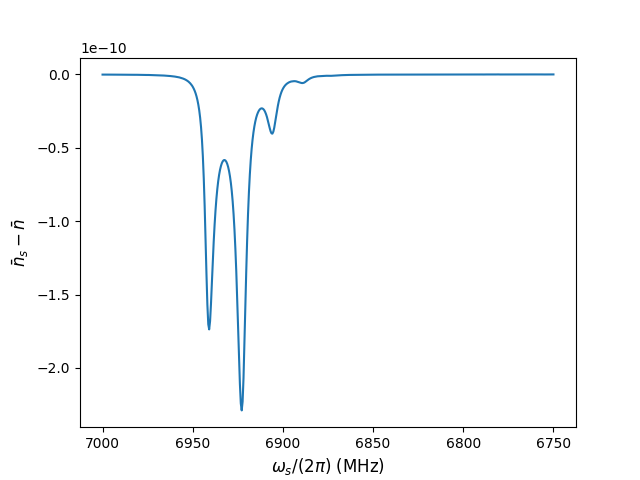
\includegraphics[width=\linewidth]{nbar_1.png}
\end{column}%
\begin{column}{0.5\linewidth}
	\centering
    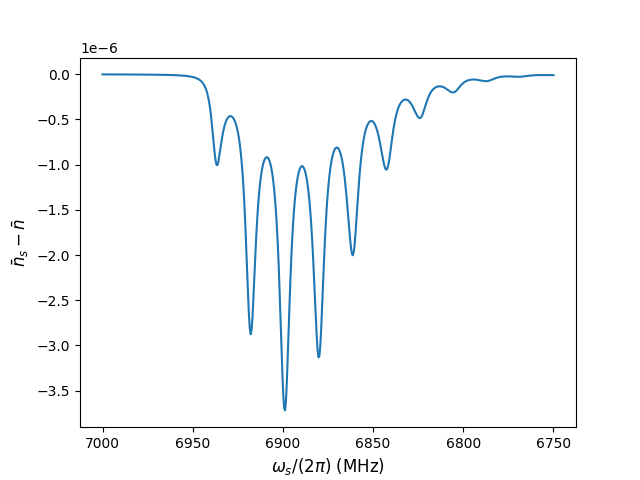
\includegraphics[width=\linewidth]{nbar_2.png}
\end{column}
\end{columns}
\end{itemize}
\end{frame}

\begin{frame}[t]\frametitle{What happens}
\begin{itemize}
	\item Excitation of the qubit is not the dominant effect, but the 
	polarization of the qubit, which twists the cavity photon state. 
	\item This can be shown from the difference of the Wigner function 
	(quasiprobability distribution on phase diagram) 
	with/without the signal field. 
\end{itemize}
\begin{columns}
\begin{column}{0.5\linewidth}
    \centering
    \only<1>{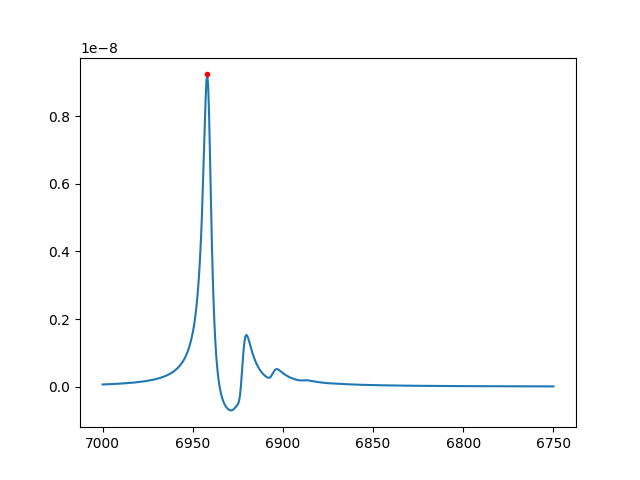
\includegraphics[width=\linewidth]{erf=0.1,point6942.png}}
    \only<2>{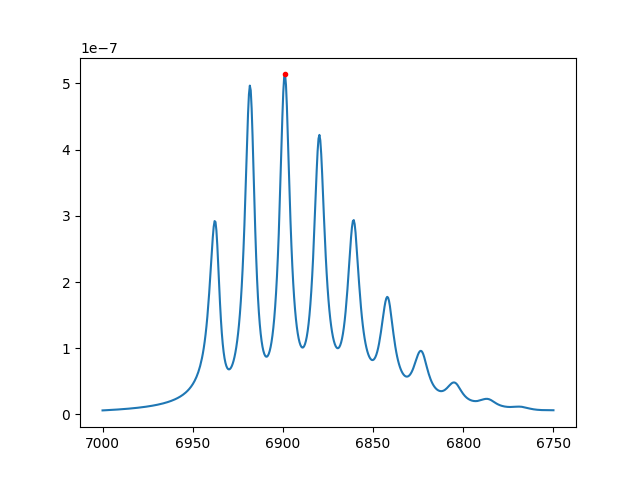
\includegraphics[width=\linewidth]{erf=20,point6898.8.png}}
\end{column}%
\begin{column}{0.5\linewidth}
	\centering
    \only<1>{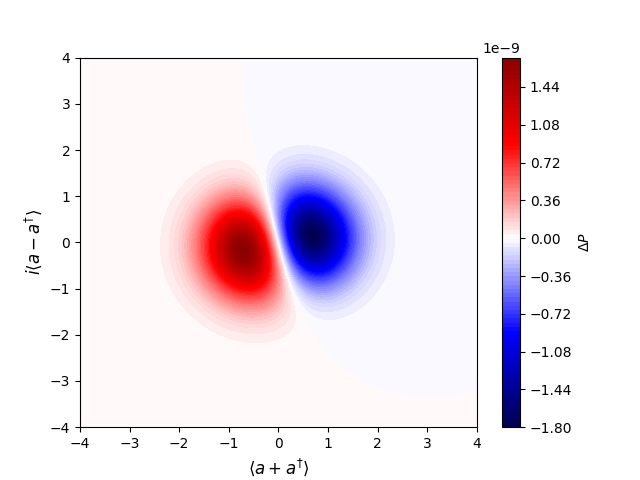
\includegraphics[width=\linewidth]{erf=0.1,point6942,wignar.png}}
    \only<2>{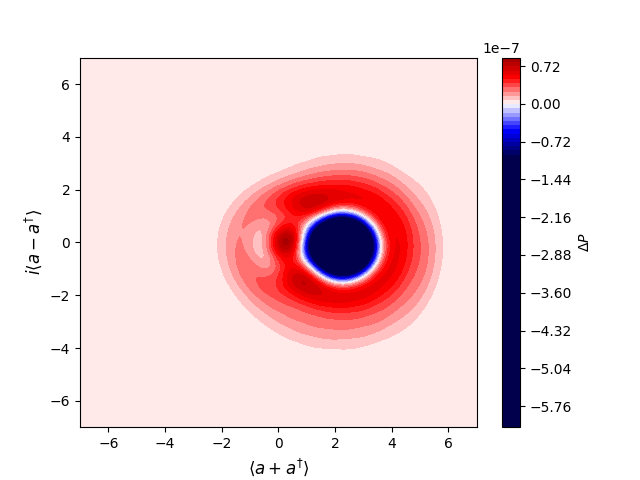
\includegraphics[width=\linewidth]{erf=20,point6898.8,wignar.png}}
\end{column}
\end{columns}
\end{frame}

\begin{frame}[allowframebreaks]
    \frametitle{Reference}
    % \printbibliography[heading=none]
    \bibliography{photonnumber}
\end{frame}

% \begin{frame}
% \centering
% \Large
% The End...\\ Thank you for listening! \\ Q \& A
% \end{frame}

\end{document}
